% Compilar desde el directorio docs/:
%   cd docs && pdflatex final.tex && pdflatex final.tex

\documentclass[11pt,a4paper]{article}

\usepackage[utf8]{inputenc}
\usepackage[T1]{fontenc}
\usepackage[spanish,es-tabla,es-noshorthands]{babel}
\usepackage{lmodern}
\usepackage[margin=2.4cm]{geometry}
\usepackage{amsmath,amssymb}
\usepackage{graphicx}
\usepackage{booktabs}
\usepackage{array}
\usepackage{tabularx}
\usepackage{caption}
\usepackage{enumitem}
\usepackage{siunitx}
\sisetup{group-separator={\,},group-minimum-digits=4}
\usepackage{xcolor}
\usepackage{hyperref}

\graphicspath{{figures/}}

\hypersetup{
  colorlinks=true,
  linkcolor=black,
  urlcolor=blue!60!black,
  citecolor=black
}

\setlength{\parskip}{0.5em}
\setlength{\parindent}{0pt}

\begin{document}

% =====================================================================
\begin{titlepage}
  \centering
  \vspace*{1.2cm}

  
\includegraphics[width=0.5\linewidth]{uniandes-logo.png}\\[1.5cm]

  {\large Facultad de Ingeniería\par}
  \vspace{0.15cm}
  {\normalsize Maestría en Inteligencia Artificial (MAIA)\par}
  \vspace{0.15cm}
  {\normalsize Aprendizaje por Refuerzo\par}

  \vspace{2.0cm}

  \rule{0.85\linewidth}{0.5pt}\\[0.6cm]
  {\LARGE \textbf{Entrega final}\par}
  \vspace{0.3cm}
  {\Large Agente Q-learning tabular sobre MiniGrid-BlockedUnlockPickup-v0\par}
  \vspace{0.6cm}
  \rule{0.85\linewidth}{0.5pt}

  \vspace{1.8cm}

  {\large Juan David Lara Camacho\par}
  \vspace{0.15cm}
  {\large Agustín Serrano\par}

  \vspace{1.0cm}

  {\normalsize Universidad de los Andes\par}
  {\normalsize \today\par}

  \vspace{1.0cm}

  \fcolorbox{gray!50}{gray!5}{%
    \begin{minipage}{0.7\linewidth}
      \centering
      \vspace{4pt}
      \small\textbf{Repositorio del proyecto}\\[0.15em]
      \href{https://github.com/JuanLara18/minigrid-qlearning}{\texttt{github.com/JuanLara18/minigrid-qlearning}}
      \vspace{4pt}
    \end{minipage}%
  }
\end{titlepage}

% =====================================================================
\begin{abstract}
\noindent
Se modela el ambiente \texttt{MiniGrid-BlockedUnlockPickup-v0} como un
proceso de decisión de Markov determinista y se entrena un agente
Q-learning tabular que lo resuelve consistentemente. La tarea exige
encadenar cinco subtareas obligatorias bajo un único inventario: mover
una bola que bloquea una puerta, recoger la llave, abrir la puerta,
soltar la llave y recoger la caja objetivo. Para que el espacio de
estados sea Markoviano sobre la función de recompensa con \emph{shaping}
por subtareas, definimos el estado como una tupla de ocho componentes
que incluye banderas de progreso persistentes. Tras \num{10000} episodios
de entrenamiento el agente alcanza \(100/100\) de éxito en evaluación
greedy con recompensa promedio \(+2.771\) (máximo teórico \(+2.80\)),
resolviendo el ambiente en \(29\) pasos.
\end{abstract}

% =====================================================================
\section{Introducción}
\label{sec:intro}

El aprendizaje por refuerzo modela un agente que interactúa con un
ambiente por medio de acciones y aprende, a partir de la recompensa que
recibe, una política que maximiza el retorno acumulado \cite{sutton}. En
el marco de los procesos de decisión de Markov (MDP) eso requiere
definir tres objetos: el conjunto de estados \(\mathcal{S}\), el
conjunto de acciones \(\mathcal{A}\) y la función de recompensa
\(R(s, a, s')\). Sobre esa formulación, Q-learning tabular
\cite{watkins} estima la función de valor estado-acción mediante
actualizaciones incrementales basadas en la ecuación de Bellman.

Este trabajo aplica el marco a un ambiente con dependencias de orden
explícitas entre subtareas: \texttt{MiniGrid-BlockedUnlockPickup-v0} de
la librería MiniGrid \cite{minigrid}. La tarea no se puede resolver sin
completar las subtareas en una secuencia fija, y la recompensa nativa
del ambiente entrega señal positiva únicamente al completar el episodio.
Eso hace necesario un diseño cuidadoso tanto del espacio de estados
como de la función de recompensa para que Q-learning tabular converja
en un número razonable de episodios.

El documento desarrolla en orden la formulación del ambiente como MDP
(Sección~\ref{sec:ambiente}), el algoritmo y los detalles de
implementación relevantes (Sección~\ref{sec:algoritmo}), la
configuración y observaciones del entrenamiento
(Sección~\ref{sec:entrenamiento}), la evaluación de la política
aprendida (Sección~\ref{sec:evaluacion}), el proceso de desarrollo con
las decisiones de diseño que llevaron a la formulación final
(Sección~\ref{sec:proceso}) y las conclusiones generales del trabajo
(Sección~\ref{sec:conclusiones}).

% =====================================================================
\section{Ambiente y formulación MDP}
\label{sec:ambiente}

El ambiente es una grilla rectangular con dos cuartos separados por un
muro vertical conectados por una sola casilla con puerta. El agente
parte en el cuarto izquierdo y debe llegar a una caja objetivo en el
cuarto derecho. La puerta está cerrada y necesita una llave del mismo
color. Una bola del mismo color que la puerta está justo enfrente,
bloqueando el acceso. El agente carga un único objeto a la vez, así que
para retirar la bola tiene que usar el inventario: \texttt{pickup} y
\texttt{drop}. El ambiente es determinista una vez fijada la semilla.

\subsection{Conjunto de estados}

El estado se representa como una tupla de ocho componentes:
\begin{equation}
  s = \big(\,
    \underbrace{(x, y)}_{\text{pos}},\;
    \underbrace{d}_{\text{dir}},\;
    \underbrace{c}_{\text{carrying}},\;
    \underbrace{b}_{\text{ball\_moved}},\;
    \underbrace{k_p}_{\text{key\_picked}},\;
    \underbrace{o}_{\text{door\_open}},\;
    \underbrace{k_d}_{\text{key\_dropped}},\;
    \underbrace{x_p}_{\text{box\_picked}}
  \,\big)
  \label{eq:state}
\end{equation}
La Tabla~\ref{tab:state} describe cada componente.

\begin{table}[h]
  \centering
  \small
  \setlength{\extrarowheight}{2pt}
  \begin{tabularx}{\linewidth}{l l l X}
    \toprule
    \textbf{Componente} & \textbf{Tipo} & \textbf{Rango} & \textbf{Descripción} \\
    \midrule
    \texttt{pos}          & \((\mathbb{Z}_{\ge 0})^2\) & \((0..W{-}1, 0..H{-}1)\) & posición del agente en la grilla \\
    \texttt{dir}          & \(\mathbb{Z}\) & \(\{0,1,2,3\}\) & orientación: 0 E, 1 S, 2 W, 3 N \\
    \texttt{carrying}     & cadena & \(\{\text{none, key, ball, box}\}\) & objeto que el agente carga en el momento actual \\
    \texttt{ball\_moved}  & booleano & \(\{0,1\}\) & la bola ya no está en su posición inicial \\
    \texttt{key\_picked}  & booleano & \(\{0,1\}\) & el agente recogió la llave en algún momento del episodio \\
    \texttt{door\_open}   & booleano & \(\{0,1\}\) & la puerta está abierta \\
    \texttt{key\_dropped} & booleano & \(\{0,1\}\) & el agente soltó la llave después de abrir la puerta \\
    \texttt{box\_picked}  & booleano & \(\{0,1\}\) & el agente cargó la caja al menos una vez \\
    \bottomrule
  \end{tabularx}
  \caption{Componentes del estado. Las cinco primeras son observables
  directamente del ambiente. Las tres últimas son banderas de progreso
  persistentes (una vez activan no vuelven a cero) y se incluyen para
  que la recompensa con \emph{shaping} (Sección~\ref{sec:recompensa})
  sea Markoviana sobre \((s, a, s')\).}
  \label{tab:state}
\end{table}

Las primeras cinco componentes son las directamente observables del
ambiente: la posición y la orientación fijan qué celda mira el agente,
y \texttt{carrying} junto con \texttt{ball\_moved} y \texttt{door\_open}
describen el estado físico relevante para decidir la siguiente acción.
Las tres últimas (\texttt{key\_picked}, \texttt{key\_dropped} y
\texttt{box\_picked}) parecen redundantes pero son indispensables para
la función de recompensa: el \emph{shaping} entrega cada bonificación
una sola vez por episodio, así que sin estas banderas la misma
transición \((s, a, s')\) podría producir recompensas distintas según
la historia previa, lo que rompería la propiedad Markoviana del modelo.

El tamaño teórico del espacio, tomando todos los productos cartesianos
posibles, es \(W \cdot H \cdot 4 \cdot 4 \cdot 2^5\), del orden de
\(10^4\) para la grilla por defecto (aproximadamente \(11\times 6\)).
La cota es laxa: las restricciones de consistencia entre banderas
(\(\texttt{key\_dropped}=1\) implica \(\texttt{door\_open}=1\) y
\(\texttt{key\_picked}=1\), y \(\texttt{box\_picked}=1\) implica las
tres anteriores) eliminan la mayoría de las combinaciones. El
entrenamiento del agente visita \num{1421} estados distintos.

\subsection{Conjunto de acciones}

El conjunto de acciones es \(\mathcal{A} = \{0,1,2,3,4,5\}\) y
corresponde a las seis acciones discretas que MiniGrid expone para este
tipo de tareas \cite{minigrid}. La Tabla~\ref{tab:actions} indica, para
cada acción, los estados en los que es aplicable y el efecto que
produce. Una acción ejecutada en un estado donde no es aplicable se
admite sin error pero deja \(s' = s\); solo avanza el contador de pasos.

\begin{table}[h]
  \centering
  \small
  \setlength{\extrarowheight}{3pt}
  \begin{tabularx}{\linewidth}{c l X X}
    \toprule
    \textbf{Idx} & \textbf{Nombre} & \textbf{Aplicable en} & \textbf{Efecto} \\
    \midrule
    0 & \texttt{left}    & todos los estados & \(d \mapsto (d-1) \bmod 4\) \\
    1 & \texttt{right}   & todos los estados & \(d \mapsto (d+1) \bmod 4\) \\
    2 & \texttt{forward} & estados con celda al frente transitable (vacía o puerta abierta) & avanza una celda en dirección \(d\) \\
    3 & \texttt{pickup}  & \texttt{carrying = none} y un objeto recogible al frente & \texttt{carrying} toma el tipo del objeto, la celda queda vacía \\
    4 & \texttt{drop}    & \texttt{carrying \(\neq\) none} y celda al frente vacía & deja el objeto en esa celda, \texttt{carrying} pasa a \texttt{none} \\
    5 & \texttt{toggle}  & puerta al frente y \texttt{carrying = key} & abre la puerta: \texttt{door\_open} pasa de \(0\) a \(1\) \\
    \bottomrule
  \end{tabularx}
  \caption{Acciones disponibles. Las seis acciones quedan disponibles
  en todo el espacio de estados; el agente aprende cuándo cada una tiene
  efecto y cuándo no a través del costo por paso de la
  Sección~\ref{sec:recompensa}.}
  \label{tab:actions}
\end{table}

\subsection{Función de recompensa}
\label{sec:recompensa}

La función \(R(s, a, s')\) suma tres ingredientes: un costo por paso
constante, las bonificaciones de \emph{shaping} por subtareas y la
recompensa terminal del ambiente:
\begin{equation}
  R(s, a, s') = \texttt{step\_cost} \;+\; \sum_{\ell\in\mathcal{L}} \beta_\ell\, \Delta_\ell(s, s') \;+\; r_{\text{goal}}\,\mathbb{1}\!\left[\,s' \text{ terminal}\,\right].
  \label{eq:reward}
\end{equation}
El indicador \(\Delta_\ell(s, s')\) vale 1 cuando la bandera de la
subtarea \(\ell\) pasa de \(0\) en \(s\) a \(1\) en \(s'\), y \(0\) en
cualquier otro caso. La Tabla~\ref{tab:rewards} lista los componentes.

\begin{table}[h]
  \centering
  \small
  \setlength{\extrarowheight}{2pt}
  \begin{tabular}{l r l}
    \toprule
    \textbf{Componente} & \textbf{Valor} & \textbf{Condición} \\
    \midrule
    \texttt{step\_cost}        & \(-0.001\) & cada paso, sin excepción \\
    \(\beta_{\text{ball}}\)    & \(+0.20\)  & \(b: 0\to 1\) \\
    \(\beta_{\text{key\_p}}\)  & \(+0.30\)  & \(k_p: 0\to 1\) \\
    \(\beta_{\text{door}}\)    & \(+0.50\)  & \(o: 0\to 1\) \\
    \(\beta_{\text{key\_d}}\)  & \(+0.30\)  & \(k_d: 0\to 1\) (requiere \(o=1\) y \(k_p=1\)) \\
    \(\beta_{\text{box}}\)     & \(+0.50\)  & \(x_p: 0\to 1\) \\
    \(r_{\text{goal}}\)        & \(+1.00\)  & \(s'\) terminal (caja entregada) \\
    \bottomrule
  \end{tabular}
  \caption{Componentes de la recompensa. La suma máxima por episodio,
  alcanzada cuando el agente completa todas las subtareas exactamente
  una vez y resuelve el episodio en \(N\) pasos, vale
  \(2.80 - 0.001\,N\).}
  \label{tab:rewards}
\end{table}

La motivación del \emph{shaping}: la recompensa nativa del ambiente
solo es positiva al recoger la caja y vale \(0\) en cualquier otro
paso. Para Q-learning tabular eso es problemático: mientras el agente
no logre por azar toda la cadena de subtareas en un mismo episodio, no
recibe ninguna señal positiva y los Q-valores no se diferencian entre
trayectorias. En pruebas iniciales con la recompensa cruda el agente
entrenó \num{10000} episodios sin encontrar la caja una sola vez. Las
cinco bonificaciones intermedias marcan hitos verificables del estado
y dan señal útil mucho antes de que aparezca una trayectoria exitosa
completa por azar.

Los valores específicos buscan que las bonificaciones intermedias no
dominen a la recompensa terminal y que el costo por paso no las anule.
Con \texttt{max\_steps}\(=576\), un costo de paso de \(-0.01\) acumula
\(-5.76\) en un episodio largo, lo que borra la suma de los
\(\beta_\ell\); por eso lo bajamos a \(-0.001\). Las bonificaciones se
distribuyeron cualitativamente según la dificultad percibida de cada
subtarea y se ajustaron empíricamente hasta lograr convergencia
consistente.

% =====================================================================
\section{Algoritmo}
\label{sec:algoritmo}

\subsection{Q-learning tabular off-policy}

El agente usa la regla canónica de Q-learning sobre una tabla indexada
por la tupla del estado:
\begin{equation}
  Q(s, a) \;\leftarrow\; Q(s, a) + \alpha \left[\, r + \gamma\,\max_{a'} Q(s', a') - Q(s, a) \,\right].
  \label{eq:qlearn}
\end{equation}
La exploración usa una política \(\varepsilon\)-greedy con
\(\varepsilon\) que decae geométricamente desde \(1.0\) hasta un piso
\(0.05\).

\subsection{Tres detalles que no son obvios}

Tres decisiones de implementación fueron necesarias para que el agente
convergiera. No son obvias a partir de la ecuación de actualización
pero condicionan que el algoritmo aprenda una política ejecutable.

\paragraph{Bootstrap solo en \texttt{terminated}, no en \texttt{truncated}.}
La ecuación~\ref{eq:qlearn} multiplica \(\max_{a'} Q(s', a')\) por
\(\gamma\). En la implementación, ese bootstrap se anula cuando
\texttt{done=True}. La pregunta es qué cuenta como \texttt{done}. El
ambiente devuelve dos banderas: \texttt{terminated} (el episodio acabó
porque se alcanzó un estado terminal real, en nuestro caso recoger la
caja) y \texttt{truncated} (el episodio se cortó por
\texttt{max\_steps}). Tratar las dos como equivalentes hace que el
agente aprenda a evitar los estados cercanos al límite de pasos aunque
sean buenos, porque cree que la trayectoria simplemente termina ahí sin
valor futuro. Solo \texttt{terminated} debe anular el bootstrap.

\paragraph{Argmax con desempate aleatorio.}
La política greedy elige
\(a^* = \arg\max_a Q(s, a)\). Cuando varias acciones empatan en
Q-valor, lo cual es frecuente al inicio del entrenamiento y en estados
poco visitados, una implementación ingenua que devuelve siempre el
primer índice produce ciclos deterministas en la política greedy: el
agente queda atrapado en una secuencia periódica que no explora. El
desempate aleatorio entre los índices con valor máximo rompe esos
ciclos sin sesgar el aprendizaje en estados con un máximo único.

\paragraph{Shaping \emph{first-time-only} dentro del estado.}
Las bonificaciones de subtarea se entregan una sola vez por episodio.
Una implementación natural mantiene un registro externo (un diccionario
de logros) y consulta ese registro al calcular la recompensa. El
problema es que entonces la misma transición \((s, a, s')\) puede
devolver recompensas distintas según la historia previa del episodio,
lo que rompe la propiedad Markoviana. Las banderas \(k_p, k_d, x_p\)
dentro del estado resuelven esto: el indicador
\(\Delta_\ell(s, s')\) que decide si se entrega la bonificación se
construye exclusivamente a partir de \(s\) y \(s'\). El precio que se
paga es un espacio de estados más grande
(Sección~\ref{sec:proceso-compromiso}).

\subsection{Hiperparámetros}

\begin{table}[h]
  \centering
  \small
  \setlength{\extrarowheight}{2pt}
  \begin{tabularx}{\linewidth}{l l X}
    \toprule
    \textbf{Parámetro} & \textbf{Valor} & \textbf{Justificación} \\
    \midrule
    \texttt{alpha} & \(0.1\) & Tasa de aprendizaje estándar para ambientes deterministas \\
    \texttt{gamma} & \(0.99\) & Descuento alto: las subtareas están a decenas de pasos del retorno terminal \\
    \texttt{epsilon} & \(1.0 \to 0.05\) & Exploración total al inicio, mínimo residual de 5\% para no quedar pegados a un óptimo local \\
    \texttt{epsilon\_decay} & \(0.9995\) & Decaimiento geométrico lento: \(\varepsilon\) toca el piso alrededor del episodio \num{6000} \\
    \texttt{N\_EPISODES} & \num{10000} & Suficiente para convergencia estable con margen \\
    \texttt{MAX\_STEPS} & \num{576} & Coincide con el límite interno del ambiente MiniGrid \\
    \texttt{env\_seed} & \(0\) & Fija la configuración inicial del ambiente \\
    \texttt{random\_seed} & \(42\) & Fija el desempate del argmax y la exploración del agente \\
    \bottomrule
  \end{tabularx}
  \caption{Hiperparámetros del entrenamiento. Las dos semillas hacen el
  experimento exactamente reproducible.}
  \label{tab:hp}
\end{table}

% =====================================================================
\section{Entrenamiento}
\label{sec:entrenamiento}

Se entrenó al agente durante \num{10000} episodios con la configuración
de la Sección~\ref{sec:algoritmo}. La Tabla~\ref{tab:progresion}
reporta la recompensa promedio sobre los \num{500} episodios previos a
cada punto de control. La Figura~\ref{fig:learning_curve} muestra la
curva completa.

\begin{table}[h]
  \centering
  \small
  \setlength{\extrarowheight}{2pt}
  \begin{tabular}{r r r r}
    \toprule
    \textbf{Episodio} & \(\boldsymbol{\varepsilon}\) & \textbf{Recompensa promedio} & \textbf{Estados visitados} \\
    \midrule
      500 & 0.779 & \(+0.201\) & \num{1258} \\
     1000 & 0.606 & \(+1.300\) & \num{1383} \\
     1500 & 0.472 & \(+1.812\) & \num{1383} \\
     2000 & 0.368 & \(+1.531\) & \num{1386} \\
     2500 & 0.286 & \(+1.737\) & \num{1387} \\
     3000 & 0.223 & \(+1.651\) & \num{1416} \\
     3500 & 0.174 & \(+1.477\) & \num{1416} \\
     4000 & 0.135 & \(+1.300\) & \num{1416} \\
     5000 & 0.082 & \(+1.118\) & \num{1421} \\
     7500 & 0.050 & \(+2.464\) & \num{1421} \\
    10000 & 0.050 & \(+2.722\) & \num{1421} \\
    \bottomrule
  \end{tabular}
  \caption{Progresión del entrenamiento: recompensa promedio sobre los
  últimos \num{500} episodios, valor de \(\varepsilon\) y cantidad
  acumulada de estados distintos visitados. La curva no es monótona; el
  texto la describe.}
  \label{tab:progresion}
\end{table}

\begin{figure}[h]
  \centering
  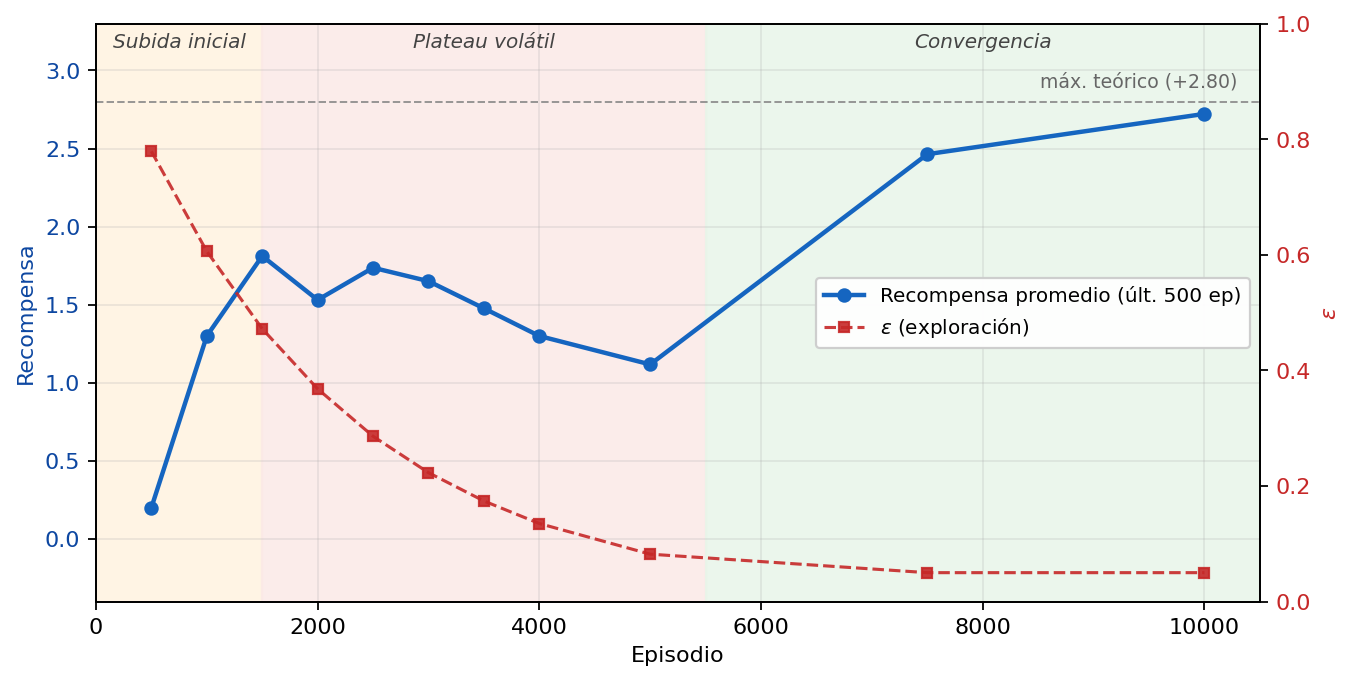
\includegraphics[width=0.92\linewidth]{final_minigrid_learning_curve.png}
  \caption{Curva de aprendizaje completa. La línea azul fina es la
  recompensa por episodio; la azul gruesa es su media móvil sobre
  \num{500} episodios. La línea punteada gris marca el máximo teórico
  \(+2.80\). La línea roja punteada (eje derecho) es \(\varepsilon\). El
  agente atraviesa una fase de \emph{plateau} volátil entre
  los episodios \num{1500} y \num{5500} antes de subir a la zona del
  máximo teórico.}
  \label{fig:learning_curve}
\end{figure}

La curva tiene tres regiones cualitativas:

\begin{description}[leftmargin=1.2cm,labelwidth=2cm,labelsep=4pt,style=nextline]
  \item[Fase 1: subida inicial (ep 1--1500).]
    \(\varepsilon\) cae de \(1.0\) a \(0.5\). La recompensa promedio
    sube de \(+0.20\) a \(+1.81\) porque el agente, todavía explorando
    fuerte, cae en las dos primeras subtareas (mover la bola, recoger la
    llave) con frecuencia creciente. Casi todo el espacio de estados
    útil aparece aquí: \num{1383} de los \num{1421} estados totales se
    ven antes del episodio \num{1500}.
  \item[Fase 2: plateau volátil (ep 1500--5500).]
    \(\varepsilon\) cae de \(0.5\) a \(\sim 0.07\) pero la recompensa
    no sube: oscila entre \(+1.1\) y \(+1.8\), incluso retrocede
    (mínimo \(+1.118\) en el episodio \num{5000}). El agente domina las
    primeras subtareas pero no encuentra de forma consistente la
    secuencia completa hasta la caja. El \(\varepsilon\) residual sigue
    siendo suficiente para que el ruido domine sobre la mejora.
  \item[Fase 3: convergencia (ep 5500--10000).]
    \(\varepsilon\) ya está en su piso de \(0.05\). La recompensa sube
    de \(+1.1\) a \(+2.72\). El agente ya tiene Q-valores estables para
    los estados raros del cuarto derecho (tras abrir la puerta) y la
    cadena completa se ejecuta consistentemente.
\end{description}

% =====================================================================
\section{Evaluación}
\label{sec:evaluacion}

\subsection{Evaluación greedy}

Tras los \num{10000} episodios de entrenamiento, se evalúa la política
greedy sobre \num{100} episodios consecutivos en el mismo ambiente con
la misma semilla. La Tabla~\ref{tab:eval_greedy} resume los números. La
Figura~\ref{fig:greedy_frames} muestra seis fotogramas equiespaciados
de un episodio greedy.

\begin{table}[h]
  \centering
  \small
  \setlength{\extrarowheight}{2pt}
  \begin{tabular}{l r}
    \toprule
    \textbf{Métrica} & \textbf{Valor} \\
    \midrule
    Tasa de éxito                          & \textbf{100 / 100} \\
    Recompensa promedio por episodio       & \(\mathbf{+2.771}\) \\
    Pasos promedio por episodio            & \(\mathbf{29.0}\) \\
    Máximo teórico de recompensa           & \(+2.80\) \\
    Pasos óptimos teóricos (cota inferior) & \(\geq 24\) \\
    \bottomrule
  \end{tabular}
  \caption{Resultados de la evaluación greedy. La diferencia entre
  \(+2.771\) y el máximo \(+2.80\) se explica por el costo acumulado de
  los pasos: \(29 \times (-0.001) = -0.029\).}
  \label{tab:eval_greedy}
\end{table}

\begin{figure}[h]
  \centering
  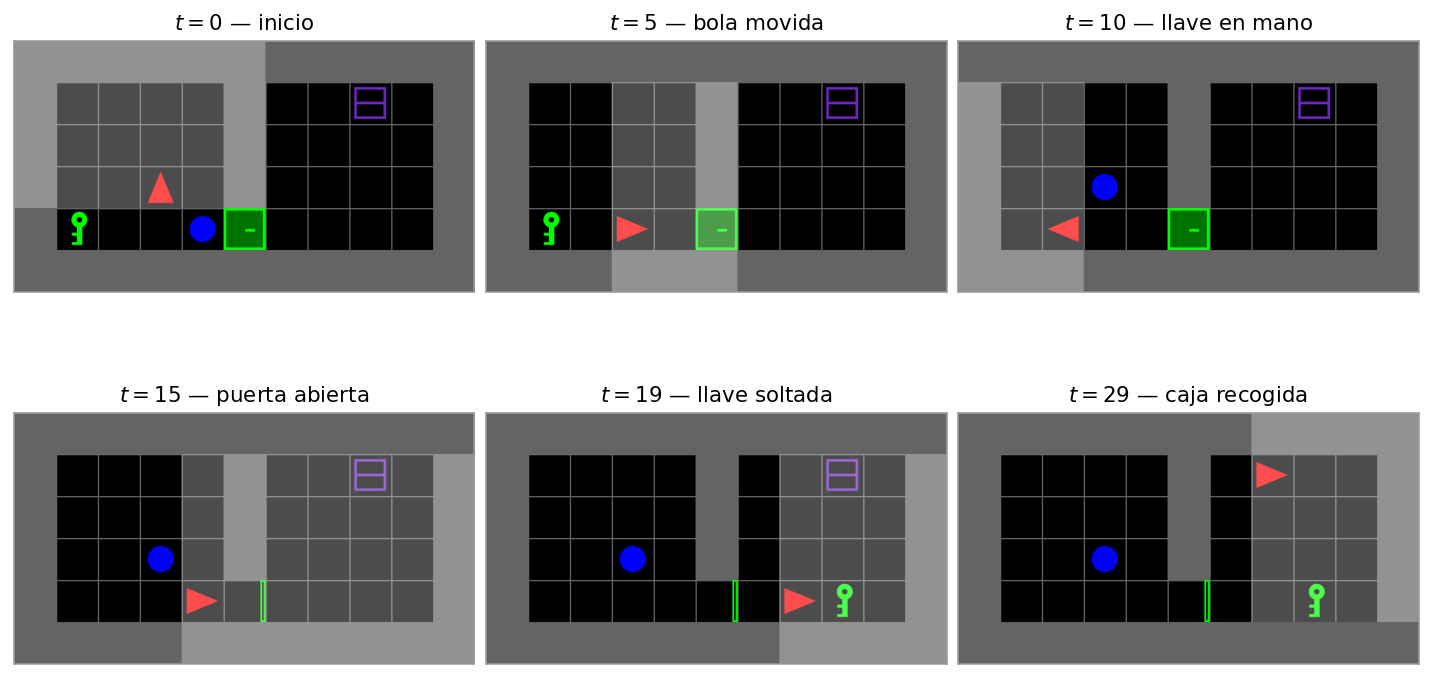
\includegraphics[width=\linewidth]{final_minigrid_greedy_frames.png}
  \caption{Seis fotogramas equiespaciados de un episodio greedy del
  agente entrenado. Fila superior: fase en el cuarto izquierdo
  (despeje de la bola, captura de la llave, acercamiento a la puerta).
  Fila inferior: cruce de la puerta, navegación en el cuarto derecho y
  recolección de la caja, que cierra el episodio.}
  \label{fig:greedy_frames}
\end{figure}

\subsection{Robustez frente a variaciones de la evaluación}

Para verificar que el resultado no depende del desempate específico del
argmax, se evaluó la misma Q-tabla con cinco semillas distintas para el
generador de números aleatorios del agente y con tres niveles de
exploración residual durante la evaluación. La
Tabla~\ref{tab:robustez} resume los resultados sobre \num{100}
episodios cada uno.

\begin{table}[h]
  \centering
  \small
  \setlength{\extrarowheight}{2pt}
  \begin{tabular}{l r r r}
    \toprule
    \textbf{Estrategia} & \textbf{Éxito} & \textbf{Reward} & \textbf{Pasos} \\
    \midrule
    Greedy, \texttt{seed=42}  & 100 / 100 & \(+2.771\) & 29.0 \\
    Greedy, \texttt{seed=0}   & 100 / 100 & \(+2.771\) & 29.0 \\
    Greedy, \texttt{seed=1}   & 100 / 100 & \(+2.771\) & 29.0 \\
    Greedy, \texttt{seed=7}   & 100 / 100 & \(+2.771\) & 29.0 \\
    Greedy, \texttt{seed=123} & 100 / 100 & \(+2.771\) & 29.0 \\
    \midrule
    \(\varepsilon\)-greedy, \(\varepsilon = 0.01\) &  99 / 100 & \(+2.750\) & 34.8 \\
    \(\varepsilon\)-greedy, \(\varepsilon = 0.05\) &  97 / 100 & \(+2.696\) & 49.4 \\
    \(\varepsilon\)-greedy, \(\varepsilon = 0.10\) &  93 / 100 & \(+2.612\) & 75.3 \\
    \bottomrule
  \end{tabular}
  \caption{Robustez. Greedy puro produce el mismo resultado bajo cinco
  semillas distintas, evidencia de que no hay empates en los estados
  visitados durante la trayectoria óptima. La degradación al introducir
  \(\varepsilon\) residual es gradual y simétrica, sin colapsos
  abruptos.}
  \label{tab:robustez}
\end{table}

% =====================================================================
\section{Proceso de desarrollo}
\label{sec:proceso}

La formulación que finalmente convergió no fue la primera que probamos.
El proceso pasó por tres versiones identificables. Esta sección las
documenta porque las decisiones que se tomaron en cada iteración
forman parte del razonamiento detrás de la solución final.

\subsection{Versión inicial: no aprende}

La primera implementación, antes del refinamiento del estado y del
shaping, presentó tasa de éxito greedy de \(0/100\) y recompensa
promedio \(-5.76\). El análisis identificó cinco problemas. La
Tabla~\ref{tab:problemas} los resume con la solución que se aplicó a
cada uno.

\begin{table}[h]
  \centering
  \small
  \setlength{\extrarowheight}{3pt}
  \begin{tabularx}{\linewidth}{l X X}
    \toprule
    \textbf{Problema} & \textbf{Causa} & \textbf{Solución aplicada} \\
    \midrule
    Estado ambiguo &
      Una bandera \texttt{has\_key} \emph{sticky} que no distinguía
      entre llevar la llave \emph{ahora} y haberla llevado en algún
      momento. Los estados ``cargo la bola'' y ``ya solté la bola''
      colapsaban. &
      Reemplazo por \texttt{carrying\_type} (cadena con el tipo de
      objeto actual), más banderas auxiliares de progreso. \\
    Costo por paso dominante &
      \(-0.01 \times 576 = -5.76\), magnitud comparable a la suma de
      los bonus de subtarea. &
      Reducido a \(-0.001\), de modo que un episodio de 576 pasos cueste
      \(-0.576\) y los bonus no queden anulados. \\
    Bootstrap incorrecto &
      \texttt{done = terminated or truncated}. El bootstrap se anulaba
      al truncar por tiempo, lo que castigaba indebidamente a las
      trayectorias largas. &
      \texttt{done} usa solo \texttt{terminated}
      (Sección~\ref{sec:algoritmo}). \\
    Ciclos en greedy &
      \texttt{argmax} devolvía siempre el primer índice empatado, lo
      que producía secuencias periódicas en estados sin política aún
      formada. &
      Desempate aleatorio entre los índices con valor máximo. \\
    Shaping incompleto &
      No había señal positiva entre abrir la puerta y recoger la caja.
      El agente abría la puerta y luego deambulaba sin saber qué
      hacer. &
      Bonus adicionales para soltar la llave (\(+0.30\)) y recoger la
      caja (\(+0.50\)). \\
    \bottomrule
  \end{tabularx}
  \caption{Los cinco problemas de la versión inicial y la solución
  aplicada en cada caso. Cada problema se diagnosticó por separado a
  partir de inspeccionar trayectorias y curvas de aprendizaje.}
  \label{tab:problemas}
\end{table}

\subsection{Versión intermedia: aprende pero no es estable}

Aplicados los fixes de estado, costo, bootstrap y desempate, el agente
empezó a aprender durante el entrenamiento (avg reward
\(\approx +1.9\) en los últimos 500 episodios) pero la evaluación
greedy seguía dando \(0/100\). La política aprendida no era ejecutable
sin la exploración residual: cuando se quitaba \(\varepsilon\), el
agente quedaba atrapado en estados del cuarto derecho que no había
visitado lo suficiente para que la Q-tabla los distinguiera.

\subsection{Versión final}

Los bonus adicionales para las subtareas finales (soltar la llave,
recoger la caja) cerraron la brecha. La política greedy se volvió
ejecutable y estable: \(100/100\) éxito, recompensa promedio
\(+2.78\). La Tabla~\ref{tab:versiones} compara las tres iteraciones.

\begin{table}[h]
  \centering
  \small
  \setlength{\extrarowheight}{2pt}
  \begin{tabular}{l r r r}
    \toprule
    \textbf{Versión} & \textbf{Reward train (últ. 500)} & \textbf{Éxito greedy} & \textbf{Reward greedy} \\
    \midrule
    Inicial      & \(\approx -5.0\) & \(0 / 100\)   & \(-5.76\) \\
    Intermedia   & \(\approx +1.9\) & \(0 / 100\)   & \(+0.42\) \\
    \textbf{Final} & \(\mathbf{\approx +2.7}\) & \(\mathbf{100 / 100}\) & \(\mathbf{+2.78}\) \\
    \bottomrule
  \end{tabular}
  \caption{Evolución entre versiones. La métrica más informativa es
  la columna ``Reward greedy'': entrena bien no implica ejecuta bien.}
  \label{tab:versiones}
\end{table}

\subsection{Un compromiso adicional: tamaño del estado}
\label{sec:proceso-compromiso}

Hubo además una decisión técnica que se tomó al pulir la solución
final, motivada por el principio Markoviano. Probamos dos
formulaciones del estado:

\begin{description}[leftmargin=0.6cm]
  \item[Formulación compacta (5 componentes)]
    \((\text{pos}, d, c, b, o)\). Las banderas \texttt{key\_picked},
    \texttt{key\_dropped} y \texttt{box\_picked} no son parte del
    estado; viven en un registro externo que el ambiente consulta al
    construir la recompensa. Espacio visitado: \num{635} estados.
    Política greedy: \(100/100\), \(+2.776\), \(24\) pasos.
  \item[Formulación markoviana (8 componentes)]
    Como en la Sección~\ref{sec:ambiente}: las tres banderas
    persistentes se incluyen en la tupla del estado. La recompensa
    \(R(s, a, s')\) queda determinada exclusivamente por \(s, s'\) sin
    consultar historia externa. Espacio visitado: \num{1421} estados.
    Política greedy: \(100/100\), \(+2.771\), \(29\) pasos.
\end{description}

El compromiso es claro. La formulación compacta entrena ligeramente más
rápido y converge a una trayectoria más corta, pero la recompensa no es
Markoviana sobre \((s, a, s')\) en el sentido estricto: la misma
transición puede dar recompensa distinta según el historial. La
formulación de 8 componentes paga un factor \(\approx 2{,}2\) en
tamaño del espacio y unos pocos pasos extra en la trayectoria, a
cambio de cumplir la propiedad Markoviana que justifica el algoritmo
de Q-learning. Optamos por la formulación de 8 componentes porque, en
un proyecto cuyo objetivo es ilustrar el marco MDP, conservar la
formalidad pesa más que ganar cinco pasos.

% =====================================================================
\section{Conclusiones}
\label{sec:conclusiones}

\begin{itemize}[leftmargin=*]
  \item Q-learning tabular resuelve completamente el ambiente cuando se
        diseña con cuidado el estado y la recompensa. Con \num{1421}
        estados distintos y seis acciones, la Q-tabla cabe holgadamente
        en memoria y converge en pocos minutos. No hizo falta función
        de aproximación.
  \item La representación del estado es la decisión más importante.
        Pasar de un flag sticky \texttt{has\_key} a un
        \texttt{carrying\_type} explícito fue lo que separó ``no
        aprende'' de ``aprende''; incluir las tres banderas
        persistentes fue lo que cerró la propiedad Markoviana.
  \item El \emph{shaping} de recompensa funciona si las bonificaciones
        marcan hitos verificables del estado (banderas que se levantan
        una sola vez), no acciones (\texttt{pickup}). Acciones son
        ambiguas; estados son no ambiguos.
  \item Algunos detalles de implementación tienen impacto outsized en
        el aprendizaje: bootstrap correcto (sólo en \texttt{terminated})
        y desempate aleatorio en el argmax fueron necesarios para que la
        política greedy fuera ejecutable.
  \item El laberinto \(8\times 7\) (Sección~\ref{sec:laberinto}) sirvió
        como referencia verificable: BFS daba la respuesta exacta y se
        pudo confirmar que el agente la igualaba. Funcionó como sanity
        check en momentos donde no estaba claro si el problema era el
        algoritmo o la formulación.
\end{itemize}

% =====================================================================
\section{Entregables y repositorio}
\label{sec:entregables}

La entrega final incluye, además de este documento, los siguientes
artefactos: la Q-tabla entrenada (\num{1416} estados con sus Q-valores
serializados), el código completo del ambiente y del agente con sus
métodos de persistencia, un video del agente resolviendo el ambiente
en \num{29} pasos, y las curvas de aprendizaje. Todo está disponible
públicamente en el repositorio del proyecto:

\begin{center}
  \fcolorbox{gray!50}{gray!5}{%
    \begin{minipage}{0.7\linewidth}
      \centering
      \vspace{6pt}
      \href{https://github.com/JuanLara18/minigrid-qlearning}{\texttt{github.com/JuanLara18/minigrid-qlearning}}
      \vspace{6pt}
    \end{minipage}%
  }
\end{center}

El \texttt{README} del repositorio detalla la estructura del código,
las instrucciones de instalación y los comandos para reproducir el
entrenamiento, la evaluación y la generación de los artefactos.

% =====================================================================
\clearpage
\appendix
\section{Trabajo adicional: laberinto rectangular \texorpdfstring{$8\times 7$}{8x7}}
\label{sec:laberinto}

\textit{En paralelo al ambiente principal trabajamos un laberinto
rectangular \(8\times 7\) con muros internos. Lo incluimos como
apéndice porque la solución óptima exacta se obtiene con BFS, lo que
dio un punto de referencia objetivo para validar la implementación de
Q-learning durante el desarrollo.}

El ambiente es una grilla de \num{8} filas por \num{7} columnas (\num{56}
celdas) con \num{37} muros internos. El agente parte en \((6, 0)\) y
debe alcanzar \((1, 6)\). El estado es \(s = (x, y)\); las acciones son
\(\mathcal{A} = \{N, S, E, W\}\) siempre aplicables; la recompensa es
\(+100\) al alcanzar la meta y \(-1\) en cualquier otro paso. Con
Q-learning tabular (\(\alpha = 0.1\), \(\gamma = 0.99\),
\(\varepsilon: 1.0 \to 0.05\) decay \(0.999\), \num{2000} episodios) el
agente alcanza \(100/100\) de éxito greedy, retorno \(+76\) y \num{25}
pasos por episodio, idéntico al camino óptimo BFS sobre el grafo
(\num{55} de \num{56} estados visitados durante el entrenamiento).

\begin{figure}[h]
  \centering
  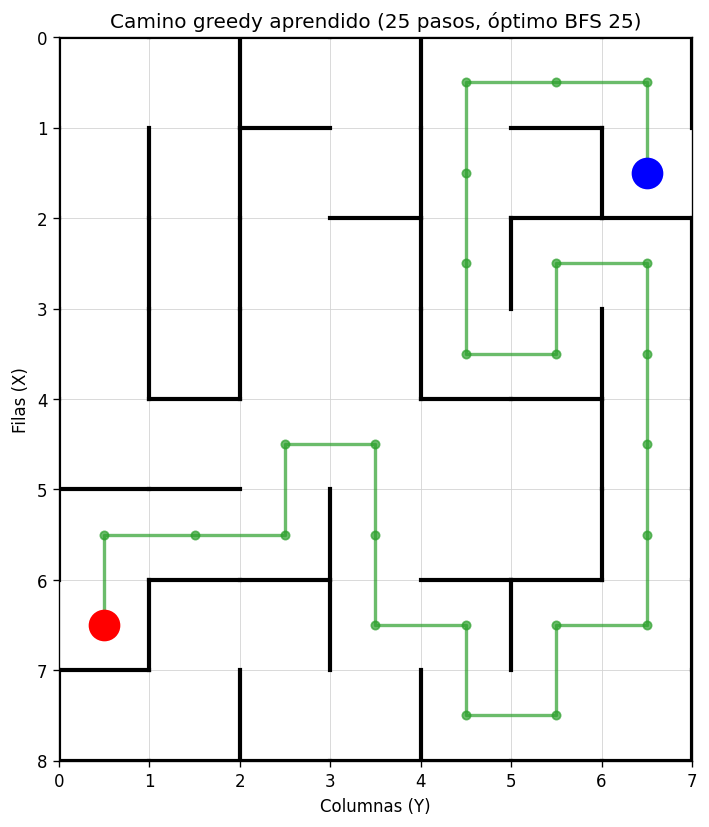
\includegraphics[width=0.42\linewidth]{maze_greedy_path.png}
  \caption{Laberinto y trayectoria greedy aprendida. Coincide con el
  óptimo BFS.}
  \label{fig:maze_path}
\end{figure}

\begin{figure}[h]
  \centering
  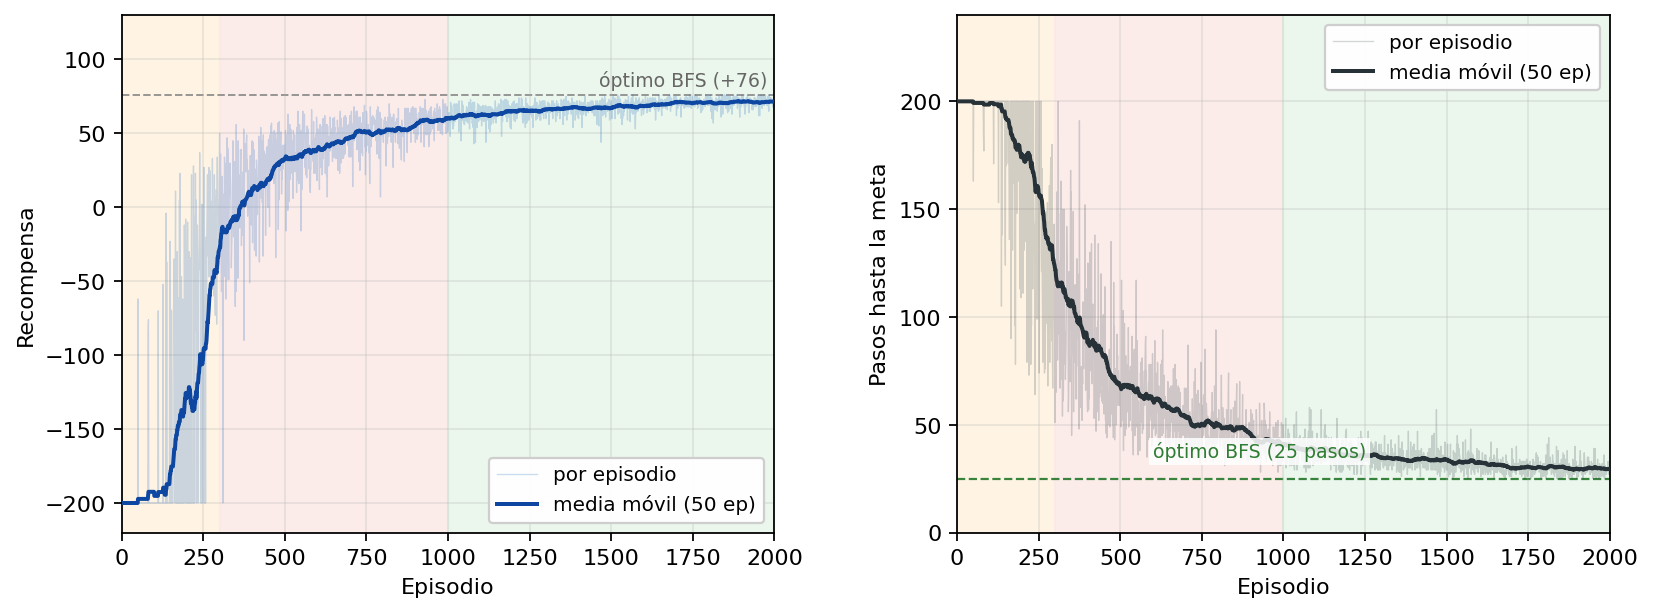
\includegraphics[width=0.95\linewidth]{final_maze_learning_curve.png}
  \caption{Curva de aprendizaje en el laberinto. Panel izquierdo:
  recompensa por episodio (línea fina cruda, línea gruesa media móvil
  de 50 episodios); la línea gris punteada en \(+76\) marca el óptimo
  BFS. Panel derecho: pasos por episodio; la línea verde punteada en
  \(25\) es el óptimo BFS. El sombreado distingue las tres fases del
  entrenamiento: caos inicial (amarillo, ep 0--300), aprendizaje rápido
  (rosa, ep 300--1000) y convergencia (verde, ep 1000--2000).}
  \label{fig:maze_lc}
\end{figure}

% =====================================================================
\clearpage
\begin{thebibliography}{9}

\bibitem{sutton}
R. S. Sutton, A. G. Barto.
\emph{Reinforcement Learning: An Introduction}.
2.\textsuperscript{a} ed., MIT Press, 2018.

\bibitem{watkins}
C. J. C. H. Watkins, P. Dayan.
``Q-learning''.
\emph{Machine Learning}, vol.~8, n.\textsuperscript{o}~3, 1992.

\bibitem{minigrid}
M. Chevalier-Boisvert, B. Dai, M. Towers, R. de Lazcano, L. Willems, S.
Lahlou, S. Pal, P. S. Castro, J. Terry.
``Minigrid \& Miniworld: Modular \& Customizable Reinforcement Learning
Environments for Goal-Oriented Tasks''.
\emph{Advances in Neural Information Processing Systems (NeurIPS)}, 2023.

\end{thebibliography}

\end{document}
